\documentclass{article}

% Language setting
% Replace `english' with e.g. `spanish' to change the document language
\usepackage[spanish]{babel}

% Set page size and margins
% Replace `letterpaper' with `a4paper' for UK/EU standard size
\usepackage[letterpaper,top=2cm,bottom=2cm,left=3cm,right=3cm,marginparwidth=1.75cm]{geometry}

% Useful packages
\usepackage{amsmath}
\usepackage{amssymb}
\usepackage[mathscr]{euscript}
\usepackage{graphicx}
\usepackage[colorlinks=true, allcolors=blue]{hyperref}

\usepackage{float}
% Keywords command
\providecommand{\keywords}[1]
{
  \small	
  \textbf{\textit{Palabras clave---}} #1
}

% //////////////////////////////////////////////////////////////
% //////////////////////////////////////////////////////////////

\title{\textbf{Protocolo de Tesis}\\Cuantificación de incertidumbre bayesiana aproximada en problemas inversos de ODE}
\author{César Isaí García Cornejo \\
Asesor: Dr. José Andrés Christen Gracia}

\begin{document}
\maketitle

\keywords{Cuantificación de incertidumbre, problema inverso, inferencia bayesiana, ecuaciones diferenciales, MCMC}

\section{Introducción}

Los fenómenos de la naturaleza son intrínsecamente causales. Las causas; que son las condiciones, cambios o variables; afligen una reacción a la cual llamamos efecto. El efecto es producto enteramente de la causa. Dicho de otra forma, sin una causa no existe el efecto, por lo que estas se encuentran en un orden tanto lógico como cronológico. Asimismo, los modelos que pretendan describir los fenómenos naturales deben ser causales, respetando orden entre causa y efecto, haciendo viable la posibilidad de generar predicciones elocuentes. 

Típicamente, los modelos matemáticos precisan de condiciones iniciales, parámetros u otras formas de variables para determinar unívocamente el problema cuya resolución propicia a la predicción de una o más cualidades del fenómeno modelado. Decimos que aquellas variables previas son las causas, mientras que el efecto son las predicciones dadas por la resolución del problema matemático.
El proceso anteriormente descrito se llama problema directo o `forward problem' ya que sigue la dirección de causalidad. Sin embargo, es interesante también el problema inverso, dada ciertas observaciones de las cualidades de un fenómeno (efectos), ¿es posible calcular las causas del modelo que rige el fenómeno?

El problema inverso es uno de los problemas matemáticos más importantes para la ciencia, debido a que ayuda a dilucidar valores de parámetros que no se pueden medir directamente. Además de que tiene un amplio campo de aplicación, entre ellos: óptica, acústica, procesamiento de señales, imágenes medicas, geofísica, oceanografía, astronomía, aprendizaje máquina y un largo etc. A pesar de su gran variabilidad de aplicaciones del problema inverso, las vicisitudes de este lo hacen un problema complejo. Mientras que el forward problem tiene solución única (en caso determinista) el problema inverso no necesariamente. Aunado al hecho de que las observaciones conllevan incertidumbre por errores de medición. Por lo anterior, es que es necesario hacer explícito toda la información a priori de los parámetros del modelo al igual que la aceptable representación de las incertidumbres en los datos.

La teoría más general se obtiene tras representar la información a priori del modelo por una distribución de probabilidad sobre el espacio de modelos, llamada distribución a priori. Dicha formulación se engloba en la estadística bayesiana, que muestra como se transforma la distribución a priori tras la consideración de las observaciones relacionadas al modelo de interés, dando la denominada distribución posterior. La metodología usual para obtener estimaciones de los parámetros se da tras la simulación de realizaciones de la distribución a posterior por métodos monte carlo, siendo el más famoso MCMC Metropolis-Hastings \cite{robert1999monte}. 


\section{Antecedentes}

% intro aquí

Sea $\mathfrak{S}$ un sistema físico bajo estudio. Ya sea $\mathfrak{S}$ una galaxia para un astrofísico, el planeta Tierra para un geofísico, o una partícula cuántica para un físico cuántico. 
El procedimiento para el estudio de un sistema físico puede ser dividido en los siguientes tres pasos. 
\begin{enumerate}
    \item Parametrización del sistema: descubrimiento del conjunto mínimo de parámetros del modelo cuyos valores caracterizan completamente el sistema.
    \item Modelación directa (forward modeling): Descubrimiento de las leyes físicas que nos permiten hacer predicciones, dado valores de parámetros del modelo, de mediciones en observables físicas.
    \item Modelación inversa: Usar las mediciones de las observables físicas para inferir los valores de los parámetros del modelo.
\end{enumerate}
Existe una fuerte retroalimentación entre estos pasos. Mientras que los primeros dos pasos son inductivos, el tercero es deductivo. Esto significa que las reglas de razonamiento que se siguen en los primeros dos pasos son difíciles de hacer explícitas. En contraste con la teoría matemática donde la lógica aplica bien en el tercer paso \cite{tarantola2005inverse}. 

\subsection{Espacio del modelo y espacio de datos} 

La elección de los parámetros de los modelos suele no ser única. Dos parametrizaciones diferentes de dicen que son equivalentes si existe una biyección que las relaciona.

Independientemente de la parametrización, es posible introducir un espacio de puntos, una variedad, donde cada punto representa un modelo del sistema. La variedad es llamada el espacio del modelo y se denota por $\mathfrak{M}$. Modelos individuales son puntos del espacio del modelo y se denotan por $\mathscr{M}_1, \mathscr{M}_2, ...$. Sin embargo, antes de preguntarse si el espacio del modelo es lineal, más importante es la distribución de probabilidad sobre este espacio. Una probabilidad sobre $\mathfrak{M}$ es el mapeo que para cualquier subconjunto $\mathcal{A}$ de $\mathfrak{M}$, llamada probabilidad de $\mathcal{A}$, con $\mathbb{P}\left (\mathfrak{M} \right ) = 1 $. Tal distribución de probabilidad puede ser definida sobre cualquier variedad finito dimensional $\mathfrak{M}$ e independientemente de cualquier parametrización de $\mathfrak{M}$.

Para obtener información en los parámetros del modelo, es necesario obtener observaciones de las observables físicas en el experimento. Podemos definir el espacio de datos como el espacio de todas las posibles respuestas del instrumento de medición. Esto corresponde a otra variedad que se representa por el símbolo $\mathfrak{D}$. Cualquier resultado de las mediciones corresponde entonces, a un punto $\mathscr{D}$ del espacio $\mathfrak{D}$ \cite{tarantola2005inverse}.



\subsection{Problema directo (forward problem)}

Los experimentos sugieren teorías físicas, y las teorías físicas predicen los resultados de los experimentos. La comparación entre la predicción y las observaciones son evidencia de la factibilidad de la teoría.

Tomando una perspectiva simplista, resolver el problema directo significa predecir los valores de las observables físicos sin error $\mathbf{d}$ que corresponde a un modelo $\boldsymbol{\theta}$. Esta predicción se denota por 
\begin{align*}
    \boldsymbol{\theta} \:\:\:\:\: \mapsto \:\:\:\:\: \mathbf{d} = \mathbf{F(\boldsymbol{\theta})}
\end{align*}
donde $\mathbf{d} = \mathbf{F(\boldsymbol{\theta})} $ es la notación reducida para $ d ^i = F^i(\theta^1,\theta^2,...)$ (i = 1,2,...) con $\theta_i$ y $d_i$ coordenadas en su respectivo espacio. El operador $F(\cdot) $ se llama operador forward y expresa el modelo matemático del sistema físico estudiado.

Los valores predichos no serán, en general, idénticos a los valores observados por las ya mencionas complicaciones: incertidumbre de las mediciones e imperfecciones del modelo. Estas dos diferentes fuentes de error producen incertidumbre del mismo orden de magnitud, debido a que tan pronto como la investigación científica progresa, los métodos experimentales decrecen la incertidumbre en sus mediciones \cite{tarantola2005inverse}.

\subsection{El método bayesiano}    

La metodología tradicional para abordar el problema inverso es por medio de la inferencia bayesiana. Dicho método se sigue de la siguiente manera:
\begin{enumerate}
    \item Elegimos una densidad para los parámetros $f(\theta) $ llamada distribución a priori, expresa la certidumbre que se tiene acerca del parámetro $\theta$ antes de observar los datos.
    \item Se selecciona el modelo estadístico $f(x|\theta)$ que refleja la certidumbre de $x$ dado $\theta$.
    \item Despues de observar los datos $X_1,...,X_n$, actualizamos la incertidumbre calculando la distribución posterior $f(\theta|X_1,...,X_n)$.
\end{enumerate}

El tercer paso de está metodología se obtiene del Teorema de Bayes, sin embargo suele ser que la distribución posterior es conocida salvo una constante de normalización. Dicha problema dificulta la posibilidad de dar estimadores analíticos. De esta forma es que entran Markov Chain Monte Carlo (MCMC) para hacer simulaciones de la distribución posterior, obteniendo estimaciones de la propia distribución así como estimaciones puntuales de los parámetros del modelo \cite{wasserman2004all}. En la próxima sección se ahondará más en los detalles.


\section{Planteamiento del problema}    


Se propone implementar por medio de código una completa resolución al problema inverso para varios modelos físicos establecidos por ecuaciones diferenciales ordinarias. Dicha implementación propone la investigación por medio de experimentación numérica para disminuir el costo de computación al resolver ecuaciones diferenciales por cada parámetro en el espacio de parámetros. Para dicho fin, se propone usar métodos análogas a k-vecinos más cercanos para la estimación de la ecuación diferencial. Los detalles de la propuesta se presentan en las siguientes secciones.

\subsection{Consideraciones generales}

En un amplio catalogo de modelos físicos, nos encontramos que gran proporción de modelos se basan en ecuaciones diferencial ordinarias dependientes de al menos un parámetro. Consideremos un modelo de este tipo. El forward problem consiste en dar un valor del parámetro o parámetros, para posteriormente resolver la ecuación diferencial. Entonces la trayectoria o solución de la ecuación diferencial será la predicción del modelo, y la causa será el valor de los parámetros.

Consideremos ahora que tenemos pares de observaciones puntuales de una trayectoria que se rige por el modelo establecido por la ODE $d_i, (i = 1,...,n)$. Pensemos que son medidas de la trayectoria de una partícula cuya posición evoluciona en el tiempo. Entonces, cada observación $d_i = (x_i, t_i)$ donde interpretamos a $x_i$ como la posición de la partícula al tiempo $t_i$. Tomemos la discretización del forward map $F_\theta(t_i)$ para el valor del forward map evaluado en el parámetro $\theta$ para el tiempo $t_i$. 


Una vez que se ha establecido el forward map es necesario esclarecer como será la incertidumbre por errores de medición así como de deficiencias del modelo, en las observaciones de los datos. 

La manera usual para establecer el error es mediante la siguiente ecuación
\begin{align}
    x_i = F_\theta (t_i) + \varepsilon_i, \:\:\:\:\: i = 1,...,n
    \label{3.01}
\end{align}
La ecuación (\ref{3.01}) para los errores representa que las diferencias entre lo observado y lo predicho tienen dependencias lineales. Consideramos que la distribución de los errores sigue un distribución normal. Es decir,
\begin{align}
    \varepsilon \sim N(0,\sigma^2)
    \label{3.02}
\end{align}

Una estructura alterna para las diferencias entre lo predicho y lo observado sigue la siguiente formulación:
\begin{align*}
    x_i = F_{\theta}(t_i + \varepsilon_i)
\end{align*}
sin embargo, tal formulación conlleva otras complicaciones por lo que se encuentra en segundo plano de la implementación.

Sea $\theta = (\theta_1, ...,\theta_m)$ los $m$ parámetros de los cuales depende el modelo a considerar. Por la metodología bayesiana es necesario dar una mediad de la certidumbre para cada parámetro. Es decir se considera que los parámetros provienen de una variable aleatoria $\Theta = (\Theta_1, ..., \Theta_m)$ y según la información a priori del modelo se propone explícitamente la distribución a prior $\pi_{\Theta}(\theta)$. Por supuesto, las variables entre parámetros son independientes, es decir podemos escribir
\begin{align*}
    \pi_{\Theta}(\theta) = \pi_{\Theta_1}(\theta_1) \cdot ... \cdot \pi_{\Theta_m}(\theta_m)
\end{align*}

En consecuencia, para el calculo de la distribución posterior solo hace falta calcular la verosimilitud del modelo en (\ref{3.01}). De la ecuación (\ref{3.01}) y (\ref{3.02}) se sigue que
\begin{align*}
    x_i \sim N(F_\theta(t_i), \sigma^2)
\end{align*}
por tanto, la verosimilitud es
\begin{align*}
    \mathcal{L}(\theta|x^n) &= \prod_{i=1}^n \frac{1}{\sqrt{2\pi \sigma^2}} e^{-\frac{1}{2\sigma^2}\left(x_i - F_{\theta}(t_i)\right)^2 } \\
    &= \left(\frac{1}{2\pi\sigma^2}\right)^{n/2} e^{\frac{1}{2\sigma^2} \sum_{i =1}^{n}\left(x_i - F_{\theta}(t_i)\right) ^2} 
\end{align*}
donde $x^n$ denota $(x_i,..., x_n)$.


Obteniendo así, la distribución posterior 
\begin{align*}
    \pi(\theta|x^n) &\propto \mathcal{L}(\theta|x^n) \pi_{\Theta}(\theta)\\
    & \propto \left(\frac{1}{2\pi\sigma^2}\right)^{n/2} e^{\frac{1}{2\sigma^2} \sum_{i =1}^{n}\left(x_i - F_{\theta}(t_i)\right) ^2} \pi_{\Theta_1}(\theta_1) \cdot ... \cdot \pi_{\Theta_m}(\theta_m)
\end{align*}
de donde una vez dada las distribuciones a priori, es posible simular variables aleatorias con dicha distribución y así obtener estimaciones de los parámetros del modelo. Dicha simulación se plantea obtener por medio de MCMC Metropolis-Hastings. Finalmente, de la simulación de la distribución posterior, se dan estimaciones puntuales de los parámetros.

\subsection{Ejemplo}

Se plantea dar una par de modelos dados por ODE's con parámetros del modelo. Uno de los modelos propuestos para resolver el problema inverso es el dado por la caída de una partícula en un campo gravitatorio constante sujeto a una fuerza de fricción dada por la dinámica clásica. La trayectoria de la partícula $x(t)$ satisface la segunda ley de Newton
\begin{align}
    m\ddot{x} = g - b \dot{x}
    \label{3.05}
\end{align}
donde $g$ es la constante de gravitación y $b$ es la constante de fricción. Estas son los parámetros del modelo. El problema forward consiste en dar valores al par de parámetros de modelos y obtener la trayectoria de la posición resolviendo la ecuación diferencial. Por simplicidad se considera de (\ref{3.05}) a $m =1$ y con las condiciones inicial $x(0)  = \dot{x}(0) = 0$.

Los datos los obtenemos de simulación, tomaremos dos valores de parámetros $g,b$ y aplicaremos el forward map para obtener puntos en la trayectoria a la cual se procede a agregar ruido gaussiano (Fig. \ref{Fig. 01}).

\begin{figure}[H]
    \centering 
    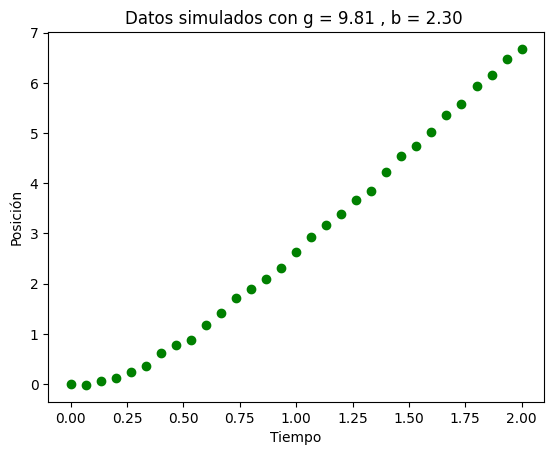
\includegraphics[width = 8 cm]{Figures/datos.png} 
    \caption{Datos simulados para caída sujeto a fricción.}
    \label{Fig. 01}
\end{figure} 

Las distribuciones a priori tienen que tener soporte en los positivos, por ello es que se proponen a ambos parámetros del modelo con distribuciones gama. Posteriormente, usando Metropolis-Hastings se se genera una caminata aleatoria en el espacio de parámetros del modelo, donde a cada paso resuelve el problema forward para los parámetros donde se encuentra la camina y así evaluar lo distribución posterior (Fig. \ref{Fig. 02})

\begin{figure}[H]
    \centering 
    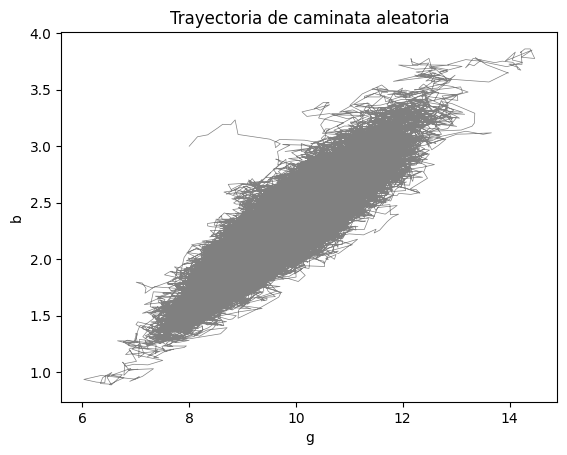
\includegraphics[width = 8 cm]{Figures/trayectoria.png} 
    \caption{Trayectoria de la caminata aleatoria del MCMC en el espacio de parámetros.}
    \label{Fig. 02}
\end{figure} 

Con la simulación de la distribución posterior, mostrada en las Fig. \ref{Fig. 3.03} y \ref{Fig. 3.04} podemos tomar el estimador de Bayes como la media de la distribución, siendo está la estimación para los parámetros.

\begin{figure}[H]
    \centering 
    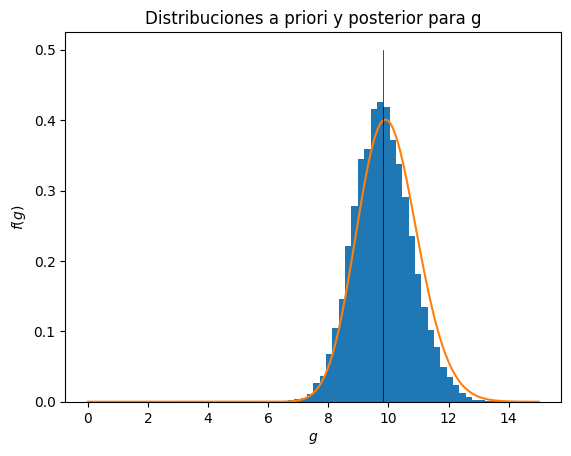
\includegraphics[width = 8cm ]{Figures/g.png}    
    \caption{Distribución a priori y distribución posterior para el parámetro g}
    \label{Fig. 3.03}
\end{figure} 


\begin{figure}[H]
    \centering 
    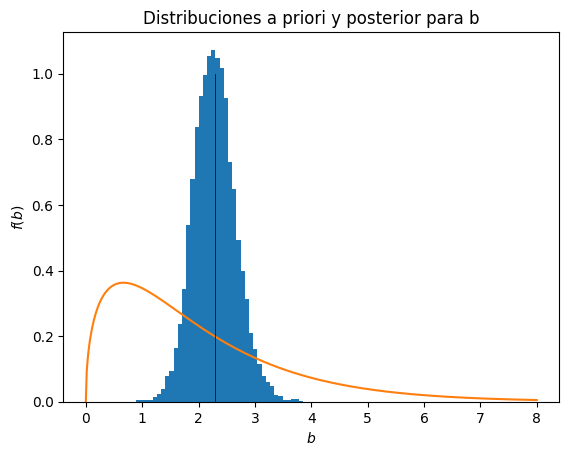
\includegraphics[width = 8cm ]{Figures/b.png}    
    \caption{Distribución a priori y distribución posterior para el parámetro b}
    \label{Fig. 3.04}
\end{figure} 

Finalmente, se coteja la calidad de la estimación con los parámetros con los que desde un principio se simularon los datos. En la Fig. \ref{Fig. 3.05} se contrastan los datos y la curva estimada dada por el problema inverso.

\begin{figure}[H]
    \centering 
    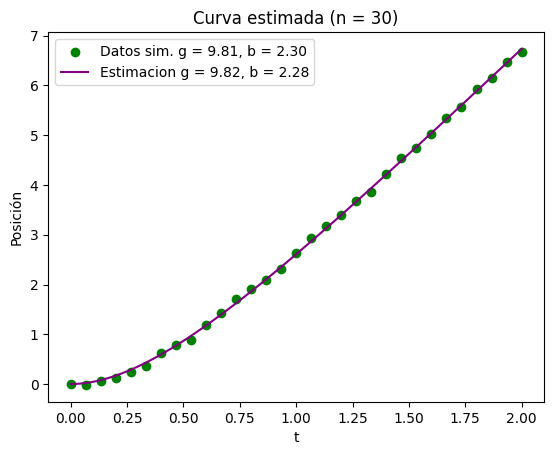
\includegraphics[width = 8 cm]{Figures/estimacion.png} 
    \caption{Estimación al problema inverso para el modelo de caída sujeto a fricción.}
    \label{Fig. 3.05}
\end{figure} 


\section{Objetivo}

A pesar de que el análisis previo nos permite obtener estimaciones bastante precisas para el problema inverso, son computacionalmente pesadas, esto debido a que a cada paso en la cadena requiere que se solucione el problema forward, es decir, se resuelven ecuaciones diferenciales tantas veces como se deje correr la cadena. 

Es así, que se desea encontrar una especie de \textit{interpolación} para solo solucionar una cantidad pequeña de veces el problema forward y para cada punto en el espacio de parámetros se pueda aproximar la solución en función de las soluciones con parámetros cercanos. (Fig. \ref{Fig. 3.06})

\begin{figure}[H]
    \centering 
    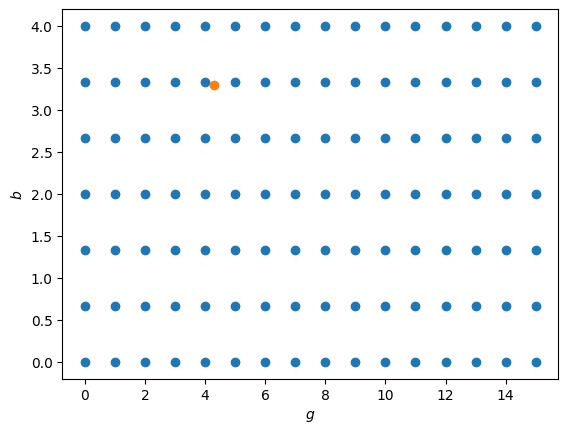
\includegraphics[width = 8 cm]{Figures/interpolacion.png} 
    \caption{Enmallado para el espacio de parámetros donde se resuelve unicamente el forward problem, cualquier punto fuera de estos se aproxima el forward map por medio de las soluciones en los puntos azules.}
    \label{Fig. 3.06}
\end{figure} 


\section{Plan de trabajo}

El plan de trabajo se subdivide en cuatro categorías: Estudio bibliográfico, implementación código, Optimización, Escritura de tesis. En el cual se subdivide el tiempo del semestre de enero a junio en las mencionadas categorías.

\begin{figure}
    \centering 
    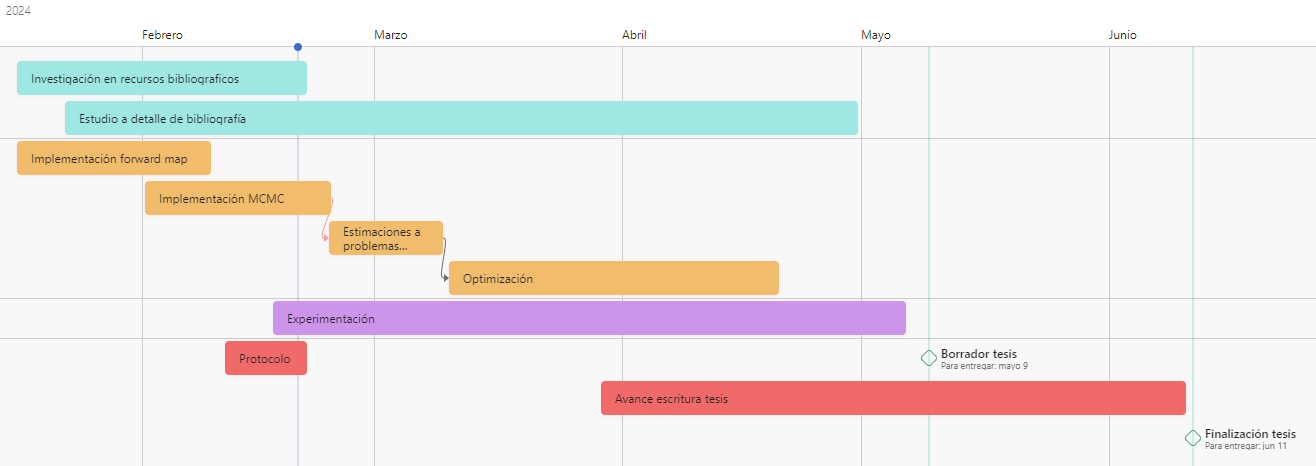
\includegraphics[width = 15 cm]{Figures/cronograma.png} 
    % \caption{}
    % \label{Fig. }
\end{figure} 


\section{Propuesta sinodales}

Dra. Lilia Leticia Ramírez Ramírez

Dr. Emilien Antoine Marie Joly (Por confirmar)

% \newpage




















% \newpage

% \vspace*{0.5}

% \section*{borrador}
% \subsection*{Introducción}

% Los fenómenos de la naturaleza manifiestan una dualidad entre causa y efecto. Entendemos por causa a las condiciones, cambios o variables que de algún modo dicha afectación conlleva a un efecto. El efecto es entonces producto enteramente de la causa. Sin una causa no existe el efecto. Nos restringimos solamente a fenómenos causales, que significa que la causa precede al efecto en un orden tanto lógico como cronológico.

% Los modelos físicos causales nos permiten hacer predicciones de un fenómeno. Dadas las causas, es posible conocer los efectos. Por fines pedagógicos, pensemos particularmente en el modelo de caída de la dinámica clásica newtoniana. Al tirar un objeto desde una altura, la gravedad actuará sobre este acelerandolo a la vez que la fuerza de fricción impide su movimiento. Por la segunda ley de Newton, la trayectoria del objeto de masa $m$ es:
% \begin{align*}
%     m\ddot{x} = g - b \dot{x}
% \end{align*}
% Las causas son la interacción de la gravedad $g$, como el coeficiente de fricción $b$. Las causas aquí son el par de parámetros $(g,b)$, y junto al modelo se pueden obtener los efectos, que es la trayectoria $x(t)$ solución de la ecuación diferencial. 

% El proceso descrito se dice que es el problema directo o `forward problem'. Sin embargo, suele ser interesante el problema inverso, es decir dado los efectos, que causas conllevo a dicho efecto. Las vicisitudes del problema inverso adolece de 







% Las vicisitudes del problema inverso radican según el modelo. Cabe la posibilidad de que para un mismo efecto existan causas diferentes que generen dicho efecto. Por ejemplo, para el modelo de gravitación newtoniano, el problema forward nos pide una distribución de masa (causa) lo que genera una fuerza a cierta partícula en el espacio (efecto). En contraste, en el problema inverso dada la fuerza ejercida en una partícula se busca encontrar la distribución de masa que generan dicha fuerza. Indudablemente, hay infinidad de soluciones al problema inverso, lo que imposibilita una clara definición del problema.


% existen infinidad de distribuciones de masa que generan la misma fuerza a dicha partícula; teniendo un problema con infinitas soluciones. Sin embargo, existen modelos en los que es posible discernir las causas de forma estimada, lo que abre la posibilidad a la inferencia estadística para abordar el problema.

% La propuesta de tesis se centra en el estudio del problema inverso para modelos descritos por ecuaciones diferenciales ordinarias bajo estadística bayesiana para estimación de parámetros dada la trayectoria observada. 

% \newpage



% \section*{Antecedentes}





% \begin{figure}
% \centering
% \includegraphics[width=0.25\linewidth]{frog.jpg}
% \caption{\label{fig:frog}This frog was uploaded via the file-tree menu.}
% \end{figure}


\bibliography{bib}{}
\bibliographystyle{plain}





\end{document}